 \documentclass[12pt]{article}
 \usepackage{cancel}
 \usepackage{multicol}
 \usepackage{amsmath}
 \usepackage{amssymb}
 \usepackage{setspace}
 \usepackage{xcolor}
 \usepackage{graphicx}    % needed for including graphics e.g. EPS, PS
 \usepackage{tikz}
 \usetikzlibrary{patterns,decorations.pathreplacing,shapes,arrows,matrix,positioning}
 \usepackage{3dplot}
 \usepackage{dsfont}
 \usepackage[vlined]{algorithm2e}
 \topmargin -2.5cm        % read Lamport p.163
 \oddsidemargin -0.04cm   % read Lamport p.163
 \evensidemargin -0.04cm  % same as oddsidemargin but for left-hand pages
 \textwidth 16.59cm
 \textheight 25.94cm
% \pagestyle{empty}        % Uncomment if don't want page numbers
 \pagenumbering{gobble}
 \parskip 7.2pt           % sets spacing between paragraphs
 %\renewcommand{\baselinestretch}{1.5} 	% Uncomment for 1.5 spacing between lines
 \parindent 0pt		  % sets leading space for paragraphs

% Title
\title{\LARGE\textbf{Chapter 8: Eigenvalues}\normalsize}

% No date in header
\date{}

\newcommand{\inv}[1]{{#1}^{-1}}

\newcommand{\iter}[1]{^{\myp{#1}}}

\newcommand{\lp}{\left(}
\newcommand{\rp}{\right)}
\newcommand{\lb}{\left[}
\newcommand{\rb}{\right]}
\newcommand{\ls}{\left\{}
\newcommand{\rs}{\right\}}
\newcommand{\lbar}{\left|}
\newcommand{\rbar}{\right|}
\newcommand{\ld}{\left.}
\newcommand{\rd}{\right.}

\newcommand{\hs}{\hspace{.75mm}}
\newcommand{\bs}{\hspace{-.75mm}}
\newcommand{\nin}{\noindent}

\newcommand{\fx}{f\bs\left( x \right)}
\newcommand{\gx}{g\bs\left( x \right)}
\newcommand{\qx}{q\bs\left( x \right)}

\newcommand{\nn}{\nonumber}

\newcommand{\vfive}{\vspace{5mm}}
\newcommand{\vthree}{\vspace{3mm}}

\newcommand{\fof}[1]{f\lp #1\rp}
\newcommand{\gof}[1]{g\lp #1\rp}
\newcommand{\qof}[1]{q\lp #1\rp}

\newcommand{\myp}[1]{\left( #1 \right)}
\newcommand{\myb}[1]{\left[ #1 \right]}
\newcommand{\myv}[1]{\left< #1 \right>}
\newcommand{\mys}[1]{\left\{ #1 \right\}}
\newcommand{\myab}[1]{\left| #1 \right|}

\newcommand{\myj}{_j}
\newcommand{\myjp}{_{j+1}}
\newcommand{\myjm}{_{j-1}}

\newcommand{\f}[1]{f\hspace{-1mm}\left( #1 \right)}
\newcommand{\fp}[1]{f'\hspace{-1mm}\left( #1 \right)}
\newcommand{\g}[1]{g\hspace{-1mm}\left( #1 \right)}
\newcommand{\gp}[1]{g'\hspace{-1mm}\left( #1 \right)}
\newcommand{\q}[1]{q\hspace{-1mm}\left( #1 \right)}
\newcommand{\qp}[1]{q'\hspace{-1mm}\left( #1 \right)}
\newcommand{\Px}[1]{P\hspace{-1mm}\left( x_{#1} \right)}
\newcommand{\Qx}[1]{Q\hspace{-1mm}\left( x_{#1} \right)}

\newcommand{\tten}[1]{\times 10^{#1}}

\newcommand{\aij}[1]{a_{#1}}
\newcommand{\bij}[1]{b_{#1}}

\newcommand{\R}[1]{\mathbb{R}^{#1}}
\newcommand{\C}[1]{\mathbb{C}^{#1}}
\newcommand{\F}[1]{\mathbb{F}^{#1}}
\newcommand{\myr}[1]{\textcolor{red}{#1}}

\newcommand{\ith}{i^{\textrm{th}}}
\newcommand{\jth}{j^{\textrm{th}}}
\newcommand{\kth}{k^{\textrm{th}}}

\newcommand{\ben}{\begin{enumerate}}
\newcommand{\een}{\end{enumerate}}

\newcommand{\beq}{\begin{eqnarray}}
\newcommand{\eeq}{\end{eqnarray}}

\tikzset{>=stealth'}

% matrix macro
\newcommand{\mymat}[1]{
\left[
\begin{array}{rrrrrrrrrrrrrrrrrrrrrrrrrrrrrrrrrrrrrrr}
#1
\end{array}
\right]
}

\newcommand{\mydet}[1]{
\left|
\begin{array}{rrrrrrrrrrrrrrrrrrrrrrrrrrrrrrrrrrrrrrr}
#1
\end{array}
\right|
}

\newcommand{\mydim}[2]{
$#1 \times #2$
}

\newcommand{\myra}{\quad \Rightarrow \quad}

\newcommand{\bS}{\mathbf{S}}
\newcommand{\bw}{\mathbf{w}}
\newcommand{\bx}{\mathbf{x}}
\newcommand{\bX}{\mathbf{X}}
\newcommand{\bd}{\mathbf{d}}
\newcommand{\bdx}{\mathbf{\delta x}}
\newcommand{\bp}{\mathbf{p}}
\newcommand{\bq}{\mathbf{q}}
\newcommand{\bz}{\mathbf{z}}
\newcommand{\bv}{\mathbf{v}}
\newcommand{\bu}{\mathbf{u}}
\newcommand{\by}{\mathbf{y}}
\newcommand{\ba}{\mathbf{a}}
\newcommand{\bb}{\mathbf{b}}
\newcommand{\bc}{\mathbf{c}}
\newcommand{\be}{\mathbf{e}}
\newcommand{\br}{\mathbf{r}}
\newcommand{\bh}{\mathbf{h}}
\newcommand{\bfb}{\mathbf{b}}
\newcommand{\xhat}{\hat{\mathbf{x}}}
\newcommand{\bzero}{\mathbf{0}}

\newcommand{\coker}{\textrm{coker}\hs}
\newcommand{\corange}{\textrm{corng}\hs}
\newcommand{\range}{\textrm{rng}\hs}
\newcommand{\myspan}{\textrm{span}\hs}
\newcommand{\rank}{\textrm{rank}\hs}
\newcommand{\trace}{\textrm{tr}\hs}

\newcommand{\lam}{\lambda}


\tikzstyle{block} = [rectangle, draw, fill=blue!15, text width=6em, text centered, rounded corners, minimum height=4em]
\tikzstyle{line} = [draw, -latex']

\tikzset{main node/.style={circle,fill=blue!20,draw,minimum size=.75cm,inner sep=0pt},
            }

% Actual document starts here
% ======================================================================================
\begin{document}
% \maketitle

% Footer
\let\thefootnote\relax\footnotetext{
\\ Chris Ketelsen
\\ CSCI 2820
\\ Lectures 21 and 22
\\ \today }

% Actual text body starts here
% ======================================================================================

\vspace{-15mm}

% =================================================================================================================
% Lecture 15: Geometry and Intro to Projections
% =================================================================================================================

\nin\Huge{\bf Lecture 21}\normalsize
\vspace{4mm}
\hrule

\vthree

\nin {\bf Recall}: We call $\lambda$ and $\bv$ ($\neq {\bf 0}$) an eigenvalue and eigenvector of a square matrix $A$ if $A\bv = \lambda \bv$.

\nin We first find the eigenvalues of a matrix by finding the roots of the {\it characteristic equation} $\det\myp{A-\lambda I} = 0$.

\nin We then find the eigenvectors of a matrix by finding the nullspace vectors of $\myp{A- \lambda I}$ for each $\lambda$.

\vthree

\nin {\bf Example 1}: Find all eigenvalues and eigenvectors of $A =
\mymat{
0 & -1 & -1 \\
1 & 2 & 1 \\
1 & 1 & 2
}$.

\vthree

\nin First we find the eigenvalues by finding the roots of $\det\myp{A - \lambda I}$.  We have

\[
\det\myp{A - \lambda I}
=
\mydet{
-\lambda & -1 & -1 \\
1 & 2-\lambda & 1 \\
1 & 1 & 2 - \lambda
}
= -\lambda \mydet{2 - \lambda & 1 \\ 1 & 2 - \lambda} - 1 \mydet{-1 & -1 \\ 1 & 2 - \lambda} + 1\mydet{-1 & -1 \\ 2 - \lambda & 1}
\]

\[
= -\lambda\mys{\myp{2-\lambda}^2 - 1} + \mys{\myp{2-\lambda}-1}+ \mys{\myp{2-\lambda}-1}
= -\myp{\lambda -1}^2\myp{\lambda -2}
\]

\vthree

\nin Setting the determininant equal to zero we see that the characteristic equation has two roots: $\lambda_1 = 1$ and $\lambda_2 = 2$.  Since the $\myp{\lambda -1}$ term in the characteristic equation has a square we call $\lambda_1 = 1$ and eigenvalue of {\it multiplicity} 2.  Since $\lambda_2 = 2$ does not appear as a square we call it a {\it simple} eigenvalue.

\vthree

\nin Next we'll find the eigenvectors associated with each eigenvalue, starting with $\lambda_1 = 1$.  We have

\[
A - 1I =
\mymat{
-1 & -1 & -1 \\
1 & 1 & 1 \\
1 & 1 & 1
}
\quad \sim \quad
\mymat{
1 & 1 & 1 \\
0 & 0 & 0 \\
0 & 0 & 0
}
\quad \Rightarrow \quad
\bx =
x_2 \mymat{-1 \\ 1 \\ 0} + x_3\mymat{-1 \\ 0 \\ 1}
\]

\vthree

\nin Notice that $\lambda_1 = 1$ is an eigenvalue of multiplicity 2 and we've found that $A - \lambda_1 I$ has two nullspace components.  Thus $\lambda_1 = 1$ has two associated eigenvectors:

\[
\bv_{1,1} = \mymat{-1 \\ 1 \\ 0} \quad \textrm{and} \quad \bv_{1,2} = \mymat{-1 \\ 0 \\ 1}
\]

\clearpage

\nin It turns out that any linear combination of $\bv_{1,1}$ and $\bv_{1,2}$ will also be an eigenvector of $A$ with associated eigenvalue $\lambda_1 = 1$.  Consider $\bv = \bv_{1,1} - 2\bv_{1,2}$.  We have

\[
A\bv =
\mymat{
0 & -1 & -1 \\
1 & 2 & 1 \\
1 & 1 & 2
}
\mymat{
1 \\
1 \\
-2
}
=
\mymat{
-1 + 2 \\
1 + 2 - 2 \\
1 + 1 - 4
}
=
\mymat{
1 \\
1 \\
-2
} \quad \checkmark
\]

\vthree

\nin We call the space $\textrm{span}\mys{\bv_{1,1}, \bv_{1,2}}$ the {\it eigenspace} associated with $\lambda_1 = 1$.

\vthree

\nin Next we find the eigenvector associated with $\lambda_2 = 2$.  We have

\[
A - 1I =
\mymat{
-2 & -1 & -1 \\
1 & 0 & 1 \\
1 & 1 & 0
}
\quad \sim \quad
\mymat{
1 & 0 & 1 \\
1 & 1 & 0 \\
-2 & -1 & -1
}
\quad \sim \quad
\mymat{
1 & 0 & 1 \\
0 & 1 & -1 \\
0 & -1 & 1
}
\]

\[
\sim \quad
\mymat{
1 & 0 & 1 \\
0 & 1 & -1 \\
0 & 0 & 0
}
\quad \Rightarrow \quad \bv_2 = \mymat{-1 \\ 1 \\ 1}
\]

\vthree

\nin Notice that despite the fact that we only found two distinct eigenvalues, the $3 \times 3$ matrix $A$ still have three linearly independent eigenvectors.  This won't happen every matrix, but it will happen the vast majority of the time.  Matrices that do not have $n$ linearly independent eigenvectors are called {\it defective}.

\vthree

\nin Here are some more interesting facts about eigenvalues:

\vthree

\nin {\bf Fact 1}: The determinant of $A$ is equal to the product of its eigenvalues.

\vthree

\nin {\bf Proof}: We know that eigenvalues are roots of the characteristic polynomial $\det\myp{A - \lambda I} = 0$.  This means that we must be able to factor the characteristic polynomial as follows:

\[
\det\myp{A - \lambda I} = \myp{\lambda_1 - \lambda}\myp{\lambda_2 - \lambda} \cdots \myp{\lambda_n - \lambda}
\]

\vthree

\nin Note that here we assume that some of the eigenvalues may have multiplicity greater than 1 and that $\lambda$ is a variable placeholder.

\vthree

\nin Then, setting $\lambda = 0$ in the characteristic equation gives  $\det A = \lambda_1\lambda_2 \cdots \lambda_n$.

\hfill $\square$

\vthree

\nin Let's check that this fact holds for the example above.  We have

\[
\det A =
\mydet{
0 & -1 & -1 \\
1 & 2 & 1 \\
1 & 1 & 2
} = 1 \mydet{1 & 1 \\ 1 & 2} - 1\mydet{1 & 2 \\ 1 & 1} = 1\myp{2 - 1} - 1\myp{1 - 2} =1 + 1 = 2
\]

\vthree

\nin Multiplying the eigenvalues (including multiplicity) gives $\lambda_{1,1}\lambda_{1,2}\lambda_2 = 1\myp{1}\myp{2} = 2 \quad \checkmark$.

\vthree

\nin The next fact requires a new matrix quantity that we haven't seen yet, the {\bf trace}.  The trace of a matrix is simply the sum of it's diagonal entries, i.e. for an $n \times n$ matrix we have

\[
\textrm{Tr}\myp{A} = a_{11} + a_{22} + \cdots + a_{nn}
\]

\vthree

\nin {\bf Fact 2}: The trace of a square matrix $A$ is equal to the sum of it's eigenvalues.

\vthree

\nin This fact is difficult to prove for an $n \times n$ matrix, so we'll just prove it for the $2 \times 2$ case.

\vthree

\nin {\bf Proof}:  Let $A = \mymat{a & b \\ c & d}$.  Then $\textrm{Tr}\myp{A} = a + d$.  Finding the eigenvalues of $A$, we have

\[
\det\myp{A - \lambda I} =
\mydet{
a - \lambda & b \\
c & d - \lambda
} = \myp{a-\lambda}\myp{d - \lambda} - bc = \lambda^2 - \myp{a + d}\lambda + \myp{ad - bc}
\]

\vthree

\nin From the quadratic equation, we have

\[
\lambda_1 = \frac{\myp{a+d} - \sqrt{\myp{a+d}^2 - 4\myp{ad-bc}}}{2} \quad \textrm{and} \quad
\lambda_2 = \frac{\myp{a+d} + \sqrt{\myp{a+d}^2 - 4\myp{ad-bc}}}{2}
\]

\vthree

\nin Summing these, we have

\[
\lambda_1 + \lambda_2 = \frac{2\myp{a+d}}{2} = a+d = \textrm{Tr}\myp{A}
\]

\hfill $\square$

\vthree

\nin Checking this with the previous example we have $\lambda_{1,1} + \lambda{1,2} + \lambda_2 = 1 + 1 + 2 = 4$ and

\[
\textrm{Tr}\myp{A} = 0 + 2 + 2 = 4 \quad \checkmark
\]

\vthree

\nin Sometimes we can deduce eigenpairs of special types of matrices.  In your homework I asked you to think about the eigenpairs of projection matrices. Here we'll look at eigenpairs of permutation matrices.

\clearpage

\nin {\bf Example 2}: Deduce the eigenpairs of $P = \mymat{0 & 1 & 0 \\ 1 & 0 & 0 \\ 0 & 0 & 1}$ without direct computation.

\vthree

\nin The action of $P$ is to swap the roles of the first and second components of a vector

\[
P\mymat{x \\ y \\ z} = \mymat{y \\ x \\ z}
\]

\vthree

\nin We want to try to think of vectors that multiplication by $P$ will leave unchanged, or scale by a constant.  One obvious one is a vector that lies along the $z$-axis.

\vthree

\[
P\mymat{0 \\ 0 \\ 1} = \mymat{0 \\ 0 \\ 1} = 1 \mymat{0 \\ 0 \\ 1} \quad \Rightarrow \quad \bv_1 = \mymat{0 \\ 0 \\ 1} \textrm{ with } \lambda_1 = 1.
\]


\tdplotsetmaincoords{70}{120}

\begin{center}
\begin{tikzpicture}[scale=2.5,
              tdplot_main_coords,
              axis/.style={thick, red,->},
              cube/.style={very thick, black},
              mydash/.style={very thin, dashed, black},
             ]

\coordinate (0) at (0,0,0);

\draw[axis] (0) -- (2.5,0,0) node[anchor=north east]{$x$};
\draw[axis] (0,0,0) -- (0,2,0) node[anchor=north west]{$y$};
\draw[axis] (0,0,0) -- (0,0,1.5) node[anchor=south]{$z$};

\draw[very thick, ->] (0,0,0) -- (0,0,1) node[right,xshift=2mm]{$\bv_1 = \mymat{0 \\ 0 \\ 1}$};

\draw (0,0,1) node[left,xshift=-2mm]{$P\bv_1$};

\end{tikzpicture}
\end{center}

\vthree

\nin Another vector that will be unchanged after multiplying by $P$ is a vector that lies in the $xy$-plane and has the same $x$- and $y$-components.  For instance

\[
P\mymat{1 \\ 1 \\ 0} = \mymat{1 \\ 1 \\ 0} = 1 \mymat{1 \\ 1 \\ 0} \quad \Rightarrow \quad \bv_2 = \mymat{1 \\ 1 \\ 0} \textrm{ with } \lambda_2 = 1.
\]


\tdplotsetmaincoords{70}{120}

\begin{center}
\begin{tikzpicture}[scale=2.5,
              tdplot_main_coords,
              axis/.style={thick, red,->},
              cube/.style={very thick, black},
              mydash/.style={very thin, dashed, black},
             ]

\coordinate (0) at (0,0,0);

\draw[axis] (0) -- (2.5,0,0) node[anchor=north east]{$x$};
\draw[axis] (0,0,0) -- (0,2,0) node[anchor=north west]{$y$};
\draw[axis] (0,0,0) -- (0,0,1.5) node[anchor=south]{$z$};

\draw[very thick, ->] (0,0,0) -- (1,1,0) node[right,xshift=2mm]{$\bv_2$};

\draw (1,1,0) node[left,xshift=-2mm]{$P\bv_2$};

\end{tikzpicture}
\end{center}

\vthree

\nin Notice that we've now found two eigenvectors with associated eigenvalue $\lambda = 1$.  This means $\lambda = 1$ is an eigenvalue with multiplicity 2, and thus has a two-dimensional eigenspace.   The eigenspace associated with $\lambda = 1$ can be described by the vertical plane that makes a 45 degree angle between the $x$- and $y$-axes.  Any vector that lies in this plane will be left unchanged by multiplying by $P$.

\tdplotsetmaincoords{70}{120}

\begin{center}
\begin{tikzpicture}[scale=2.5,
              tdplot_main_coords,
              axis/.style={thick, red,->},
              cube/.style={very thick, black},
              mydash/.style={very thin, dashed, black},
             ]

\coordinate (0) at (0,0,0);

\draw[axis] (0) -- (2.5,0,0) node[anchor=north east]{$x$};
\draw[axis] (0,0,0) -- (0,2,0) node[anchor=north west]{$y$};
\draw[axis] (0,0,0) -- (0,0,2.0) node[anchor=south]{$z$};

\draw[very thick] (0,0,0) -- (2,2,0) -- (2,2,1.5) -- (0,0,1.5) -- cycle;

\end{tikzpicture}
\end{center}

\clearpage

\nin The third and final eigenvector of $P$ is a vector that lies orthogonal to this plane.

\vthree

\nin Consider the vector $\bv_3 = \mymat{1 \\ -1 \\ 0}$.

\vthree

\[
P\mymat{1 \\ -1 \\ 0} = \mymat{-1 \\ 1 \\ 0} = -1 \mymat{1 \\ -1 \\ 0} \quad \Rightarrow \quad \bv_3 = \mymat{1 \\ -1 \\ 0} \textrm{ with } \lambda_3 = -1.
\]

\vthree

\nin The action of $P$ on $\bv_3$ is to reflect the vector across the plane formed by the eigenspace of $\lambda = 1$ resulting in the negative of $\bv_3$.

\tdplotsetmaincoords{70}{120}

\begin{center}
\begin{tikzpicture}[scale=2.5,
              tdplot_main_coords,
              axis/.style={thick, red,->},
              cube/.style={very thick, black},
              mydash/.style={very thin, dashed, black},
             ]

\coordinate (0) at (0,0,0);

\draw[axis] (0) -- (2.5,0,0) node[anchor=north east]{$x$};
\draw[axis] (0,0,0) -- (0,2,0) node[anchor=north west]{$y$};
\draw[axis] (0,0,0) -- (0,0,2.0) node[anchor=south]{$z$};

\draw[very thick, ->] (0,0,0) -- (1,-1,0) node[left,xshift=-2mm]{$\mymat{1\\-1\\0} =\bv_3$};
\draw[very thick, ->] (0,0,0) -- (-1,1,0) node[right,xshift=2mm]{$P\bv_3 = \mymat{-1 \\ 1 \\ 0}$};

\draw[thick, dashed] (0,0,0) -- (2,2,0) -- (2,2,1.5) -- (0,0,1.5) -- cycle;

\end{tikzpicture}
\end{center}

\vthree

\nin I'll leave it as an exercise for you to compute the eigenvalues and eigenvectors of $P$ directly and confirm that what we've deduced geometrically is correct.

\vthree

\nin {\bf Example 3}: Consider the matrix $Q = \mymat{0 & -1 \\ 1 & 0}$.

\vthree

\nin The action of $Q$ is to rotate a vector in $\R{2}$ ninety degrees in the counterclockwise direction.

\vthree

\begin{center}
\begin{tikzpicture}[scale=1,
                          axis/.style={thick, red,->},
                          cube/.style={very thick, black},
                          mysolid/.style={very thick, black},
                          mydash/.style={thick, dashed, black},
                         ]


\coordinate (0) at (0,0);

\draw[axis] (-3,0) -- (5,0) node[right]{};
\draw[axis] (0) -- (0,5) node[right]{};

\draw[mysolid, ->] (0,0) -- (4,2) node[right,xshift=2pt]{$\bx = \mymat{a \\ b}$};
\draw[mysolid, ->] (0,0) -- (-2,4) node[left,xshift=-2pt]{$Q\bx = \mymat{-b \\ a}$};

\draw[thick] (2pt,2)--(-2pt,2) node[left]{\footnotesize$b$\normalsize};
\draw[thick] (4,2pt)--(4,-2pt) node[below]{\footnotesize$a$\normalsize};
\draw[thick] (2pt,4)--(-2pt,4) node[left]{\footnotesize$a$\normalsize};
\draw[thick] (-2,2pt)--(-2,-2pt) node[below]{\footnotesize$-b$\normalsize};

\end{tikzpicture}
\end{center}

\clearpage

\nin Can you think of any nonzero vectors that rotation by 90 degrees counterclockwise results in a scaled version of the original vector?  I can't.

\vthree

\nin So does that mean that the matrix $Q$ has no eigenpairs?  Let's try to find them by direct computation instead of geometry.

\vthree

\[
\det\myp{Q - \lambda I} =
\mydet{
-\lambda & -1 \\
1 & -\lambda
}
= \lambda^2 + 1 = 0
\quad \Rightarrow \quad \lambda = \pm \sqrt{-1} = \pm \hs i
\]

\vthree

\nin The eigenvalues are {\bf imaginary}!  OK, this is fine.  It happens.

\vthree

\nin The associated eigenvectors also have imaginary components.  We have

\[
\lambda_1 = i  \quad \bv_1 = \mymat{i \\ 1} \quad \textrm{and} \quad
\lambda_2 = -i \quad \bv_1 = \mymat{-i \\ 1}
\]

\clearpage

\nin\Large{\bf Undirected Graphs and Their Associated Matrices}\normalsize
\vspace{4mm}
\hrule

\vthree

\nin In this lecture we'll look at a method to encode an undirected graph in a special matrix called an {\it adjacency matrix}.

\vthree

\nin Consider the following undirected graph, $G$,

\begin{center}
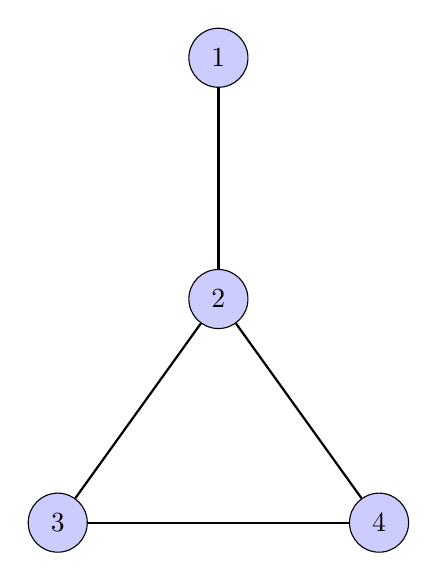
\begin{tikzpicture}

    \node[main node] (1) {$1$};
    \node[main node] (2) [below = 2.3cm of 1] {$2$};
    \node[main node] (3) [below left = 2.3cm and 1.5cm of 2]  {$3$};
    \node[main node] (4) [below right = 2.3cm and 1.5cm of 2] {$4$};

    \path[draw,thick,-]
    (1) edge node {} (2)
    (2) edge node {} (3)
    (2) edge node {} (4)
    (3) edge node {} (4);

\end{tikzpicture}
\end{center}

\vthree

\nin {\bf Def}: The adjacency matrix $A$ of an undirected graph $G$, is a square $n \times n$ matrix where $n$ is the number of vertices in the graph.  The entries of $A$ are given by

\[
A_{ij} =
\left\{
\begin{array}{rl}
1 & \textrm{if } i \leftrightarrow j \\
0 & \textrm{otherwise}
\end{array}
\right.
\]

\vthree

\nin This says that the $(i,j)$-entry of the adjacency matrix is $1$ is there is an edge connecting vertices $i$ and $j$ and $0$ if there is not.

\vthree

\nin {\bf Example 1}:  For the graph $G$ pictured above, the adjacency matrix is

\[
A =
\mymat{
0 & 1 & 0 & 0 \\
1 & 0 & 1 & 1 \\
0 & 1 & 0 & 1 \\
0 & 1 & 1 & 0 \\
}
\]

\vthree

\nin {\bf Fact 1}: The adjacency matrix $A$ of an undirected graph is always symmetric.

\clearpage

\nin {\bf Def}:  The {\bf degree} of a vertex is the number of vertices that it is connected to (or alternatively, the number of edges that it is a part of).  We denote the degree of vertex $i$ by $d_i$.

\vthree

\nin {\bf Example 2}:  For the graph $G$ pictured above the vertex degrees are

\[
d_1 = 1 \quad \quad
d_2 = 3 \quad \quad
d_3 = 2 \quad \quad
d_4 = 2
\]

\vthree

\nin {\bf Fact 2}: The degree of vertex $i$ is equal to the sum of row $i$.

\vthree

\nin {\bf Def}:  A walk is a list of vertices that can be traversed along edges in the graph.  Note that there is no restriction on the number of times a vertex is touched during a walk.

\vthree

\nin {\bf Example 3}.  Denote the $i^{\textrm{th}}$ vertex by $v_i$.  Then the walk the walk that goes from vertex 1 to vertex 2 to vertex 4 is denoted by $v_1-v_2-v_4$.  The walk that goes from vertex 1 to vertex 2 to vertex 3 and then back to vertex 2 is denoted by $v_1-v_2-v_3-v_2$.

\vthree

\nin {\bf Fact 3}:  The $(i,j)$-entry of the matrix power $A^k$ tell you how many walks of length $k$ exist in the graph that start at vertex $i$ and end at vertex $j$.

\vthree

\nin {\bf Example 4}: We'll look at powers of the adjacency matrix corresponding to the the graph $G$ pictured above.  For the first power of $A$ we have

\vthree

\nin $
A^1 =
\mymat{
0 & 1 & 0 & 0 \\
1 & 0 & 1 & 1 \\
0 & 1 & 0 & 1 \\
0 & 1 & 1 & 0 \\
}
$

\vthree

\nin This is of course just the adjacency matrix of $G$ itself.  According to Fact 3, since $A_{12} = 1$ there is exactly one walk that starts at $v_1$ and ends at $v_2$.  This is of course true because there is an edge between $v_1$ and $v_2$.  Similarly, $A_{13}=0$, indicating that there are no length-1 walks between $v_1$ and $v_3$.

\vthree

\nin Squaring the matrix $A$, we have

\vthree

\nin $
A^2 =
\mymat{
1 & 0 & 1 & 1 \\
0 & 3 & 1 & 1 \\
1 & 1 & 2 & 1 \\
1 & 1 & 1 & 2 \\
}
$

\vthree

\nin According to Fact 3, since $A_{14}=1$ there is exactly one length-2 walk that starts at $v_1$ and ends at $v_4$.  From the graph we see that this is the walk $v_1-v_2-v_4$.  Notice that it is impossible to traverse a different sequences of vertices to get from $v_1$ to $v_4$.  Similarly, since $A_{22} = 3$ there are exactly three length-2 walks that start at $v_2$ and end at $v_2$.  These are $v_2-v_1-v_2$, $v_2-v_3-v_2$, and $v_2-v_4-v_2$.

\clearpage

\nin Finally, cubing $A$ we have

\vthree

\nin $
A^3 =
\mymat{
0 & 3 & 1 & 1 \\
3 & 2 & 4 & 4 \\
1 & 4 & 2 & 3 \\
1 & 4 & 3 & 2 \\
}
$

\vthree

\nin Since $A_{42} = 4$ there are exactly four length-3 paths that start at $v_4$ and end at $v_2$.  Looking at the graph we see that these walks are $v_4-v_2-v_1-v_2$, $v_4-v_2-v_3-v_2$, $v_4-v_2-v_4-v_2$, and $v_4-v_3-v_4-v_2$.

\vthree

\nin {\bf Def}: A graph is called {\it connected} if there exists a walk from $v_i$ to $v_j$ for all pairs $i$ and $j$.

\vthree

\nin {\bf Fact 4}: A graph $G$ is connected if there exists some integer $k > 0$ such that $B_k = I + A + A^2 + \cdots + A^k$ has all positive entries.

\vthree

\nin Essentially this works because the entries of the powers of $A$ give the number of walks of length $k$ that connect each of the vertices.  If $B_k$ has all positive entries, then there exists a walk of at most length $k$ between any two vertices.

\vthree

\nin {\bf Example 5}:  For the adjacency matrix for the example graph, we have

\[
B_1 = I + A =
\mymat{
1 & 1 & 0 & 0 \\
1 & 1 & 1 & 1 \\
0 & 1 & 1 & 1 \\
0 & 1 & 1 & 1 \\
}
\]

\vthree

\nin Since there are zero entries in $B_1$ it is not the case that you can get from every vertex to every other in walks of length 1 (for instance, it's impossible to get from $v_1$ to $v_3$ in one step).

\vthree

\nin We then have

\[
B_2 = I + A + A^2 =
\mymat{
2 & 1 & 1 & 1 \\
1 & 4 & 2 & 2 \\
1 & 2 & 3 & 2 \\
1 & 2 & 2 & 3 \\
}
\]

\vthree

\nin Since $B_2$ has all positive entries we know that $G$ is connected, and you can get from any vertex to any other in a walk of length 2 or less.  This is clearly verified by looking at the graph.

\clearpage

\nin {\bf Example 6}: Consider the following disconnected graph

\vthree

\begin{center}
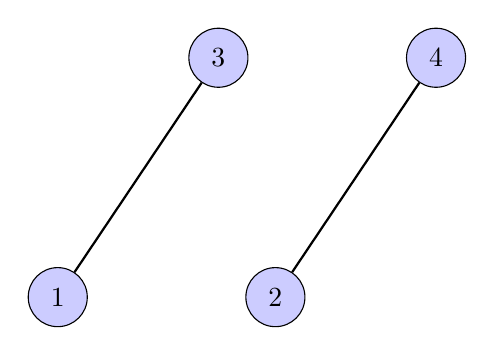
\begin{tikzpicture}

    \node[main node] (1) {$1$};
    \node[main node] (3) [above right = 2.5cm and 1.5cm of 1]  {$3$};
    \node[main node] (2) [right = 2.0cm of 1]  {$2$};
    \node[main node] (4) [above right = 2.5cm and 1.5cm of 2]  {$4$};

    \path[draw,thick,-]
    (1) edge node {} (3);

    \path[draw,thick,-]
    (2) edge node {} (4);

\end{tikzpicture}
\end{center}

\vthree

\nin The associated adjacency matrix is $A =
\mymat{
0 & 0 & 1 & 0 \\
0 & 0 & 0 & 1 \\
1 & 0 & 0 & 0 \\
0 & 1 & 0 & 0 \\
}
$

\vthree

\nin Taking powers of $A$ we have

\vthree

\[
A^2 =
\mymat{
1 & 0 & 0 & 0 \\
0 & 1 & 0 & 0 \\
0 & 0 & 1 & 0 \\
0 & 0 & 0 & 1 \\
}
\quad
\quad
A^3 =
\mymat{
0 & 0 & 1 & 0 \\
0 & 0 & 0 & 1 \\
1 & 0 & 0 & 0 \\
0 & 1 & 0 & 0 \\
}
\quad
\quad
A^4 =
\mymat{
1 & 0 & 0 & 0 \\
0 & 1 & 0 & 0 \\
0 & 0 & 1 & 0 \\
0 & 0 & 0 & 1 \\
}
\]

\vthree

\nin Clearly this pattern repeats.  Thus for any integer $k$ the matrix $B_k$ has the form

\[
B_k = I + A + A^2 + \cdots + A^k =
\mymat{
* & 0 & * & 0 \\
0 & * & 0 & * \\
* & 0 & * & 0 \\
0 & * & 0 & * \\
}
\]

\vthree

\nin Since $B_k$ will not have all positive entries for any value of $k$ the graph is not connected.

\vthree

\nin {\bf Example 7}:  Note that the analysis in Example 6 tells us that the associated graph has multiple disconnected components, but it doesn't really tell us where they are.  It turns out that we can determine the disconnected components of a graph by examinging the eigenvectors of a new graph matrix: the so-called {\bf Graph Laplacian Matrix}.  First we need a diagonal matrix $D$ called the degree matrix of an undirected graph.  It has the following form

\[
D_{ij} =
\left\{
\begin{array}{rl}
d_i & \textrm{if } i = j \\
0 & \textrm{otherwise}
\end{array}
\right.
\]

\vthree

\nin Note that this is simply a diagonal matrix whose $i^{\textrm{th}}$ main diagonal entry is the degree of vertex $i$.  The degree matrix $D$ together with the adjacency matrix $A$ allows us to construct the graph Laplacian, which we call $L$.  We have

\[
L = D - A
\]

\vthree

\nin For the graph in Example 1, we have

\[
L = D - A =
\mymat{
1 & 0 & 0 & 0 \\
0 & 3 & 0 & 0 \\
0 & 0 & 2 & 0 \\
0 & 0 & 0 & 2 \\
} -
\mymat{
0 & 1 & 0 & 0 \\
1 & 0 & 1 & 1 \\
0 & 1 & 0 & 1 \\
0 & 1 & 1 & 0 \\
}
=
\mymat{
1 & -1 & 0 & 0 \\
-1 & 3 & -1 & -1 \\
0 & -1 & 2 & -1 \\
0 & -1 & -1 & 2 \\
}
\]

\vthree

\nin Notice that the $-1's$ on the off-diagonals of $L$ correspond to entries in the adjacency matrix $A$ (i.e. they tell us which vertices are connected) and the diagonal entries of $L$ tell us the degree of each vertex.  Notice in particular that each row of $L$ sums to zero.  This must be true since the $-1$'s in row $i$ correspond to the vertices that are connected to vertex $i$, and the diagonal element is the degree of vertex $i$ (i.e. the number of nodes the vertex is connected to).

\vthree

\nin Since the rows of $L$ sum to zero, it is very easy to find an eigenvector of $L$ corresponding to a zero eigenvalue.  Any nonzero constant vector (e.g. a vector of all $1$'s) will work.  Define $\mathds{1}$ to be the vector of all $1$'s, then

\[
L \mathds{1} =
\mymat{
1 & -1 & 0 & 0 \\
-1 & 3 & -1 & -1 \\
0 & -1 & 2 & -1 \\
0 & -1 & -1 & 2 \\
}
\mymat{1 \\ 1 \\ 1 \\ 1}
= \mymat{ 0 \\ 0 \\ 0 \\0 }
=
0 \times
\mymat{1 \\ 1 \\ 1 \\ 1}
\]

\vthree

\nin  So we have $\bv = \mathds{1}$ and $\lambda = 0$ is an eigenpair of $L$.  For this particular graph, this is the only eigenvector associated with $\lambda = 0$.  The other eigenvalues are $\lambda_2 = 1$, $\lambda_3 = 3$ and $\lambda_4 = 4$.

\vthree

\nin {\bf Example 8}:  Now consider the graph Laplacian of the graph in Example 6.  We have

\[
D =
\mymat{
1 & 0 & 0 & 0 \\
0 & 1 & 0 & 0 \\
0 & 0 & 1 & 0 \\
0 & 0 & 0 & 1 \\
},
\quad
A =
\mymat{
0 & 0 & 1 & 0 \\
0 & 0 & 0 & 1 \\
1 & 0 & 0 & 0 \\
0 & 1 & 0 & 0 \\
} \quad \Rightarrow \quad
L =
\mymat{
1 & 0 &-1 & 0 \\
0 & 1 & 0 &-1 \\
-1 & 0 & 1 & 0 \\
0 & -1 & 0 & 1 \\
}
\]

\vthree

\nin Notice that, as expected, the constant vector $\mathds{1}$ is in the nullspace of $L$, and therefore is an eigenvector of $L$ with associated eigenvalue $\lambda = 0$.  It turns out though, that this graph Laplacian has a second zero eigenvalue (or we could say, $\lambda = 0$ is an eigenvalue with multiplicity 2).  If you compute the eigenvalues of $L$ (by hand, or with Matlab), you find that the eigenvalues are $\lambda_1 = 0$, $\lambda_2 = 0$, $\lambda_3 = 2$, and $\lambda_4 = 2$.  We are interested in the eigenvectors of $L$ associated with the zero eigenvalue.  Solving for those eigenvectors, we have

\[
L - 0I = L =
\mymat{
1 & 0 &-1 & 0 \\
0 & 1 & 0 &-1 \\
-1 & 0 & 1 & 0 \\
0 & -1 & 0 & 1 \\
}
\quad \sim \quad
\mymat{
1 & 0 &-1 & 0 \\
0 & 1 & 0 &-1 \\
0 & 0 & 0 & 0 \\
0 & -1 & 0 & 1 \\
}
\quad \sim \quad
\mymat{
1 & 0 &-1 & 0 \\
0 & 1 & 0 &-1 \\
0 & 0 & 0 & 0 \\
0 & 0 & 0 & 0 \\
}
\]

\clearpage

\nin Finding the two nullspace vectors (eigenvectors), we have

\[
\bv_1 = \mymat{1 \\ 0 \\ 1 \\ 0}
\quad
\bv_2 = \mymat{0 \\ 1 \\ 0 \\ 1}
\]

\vthree

\nin OK, now think of the entries of $\bv_1$ and $\bv_2$ as corresponding to the vertices on the graph.  Notice that for $\bv_1$, the nonzero entries are in the first and third positions.  If you look at the graph in Example 6, you'll see that vertices $v_1$ and $v_3$ are connected to each other, but diconnected from vertices $v_2$ and $v_4$.  Similarly, the nonzero entries in $\bv_2$ correspond to vertices $v_2$ and $v_4$.  Vertices $v_2$ and $v_4$ are connected to each other, but not connected to vertices $v_1$ and $v_2$.    In other words, each eigenvector associated with $\lambda=0$ corresponds to a particular disconnected component of the graph.

\vthree

\nin Furthermore, the graph corresponding to Examples 1 and 7 had only one eigenvector associated with $\lambda = 0$.  This is because the graph from Examples 1 and 7 is connected.

\vthree

{\bf Fact}:  The multiplicity of the $\lambda = 0$ eigenvalue of the graph Laplacian tells you the number of disconnected components in a graph.  The nonzero entries in each eigenvector corresponding to $\lambda = 0$ tells you which vertices are in the corresponding  component.


\clearpage

\nin {\bf Example 7}:  Vertices can also have self-loops.  Consider the modification of the graph in Example 1 where we add self-loops to vertices 1 and 4.

\vthree

\begin{center}
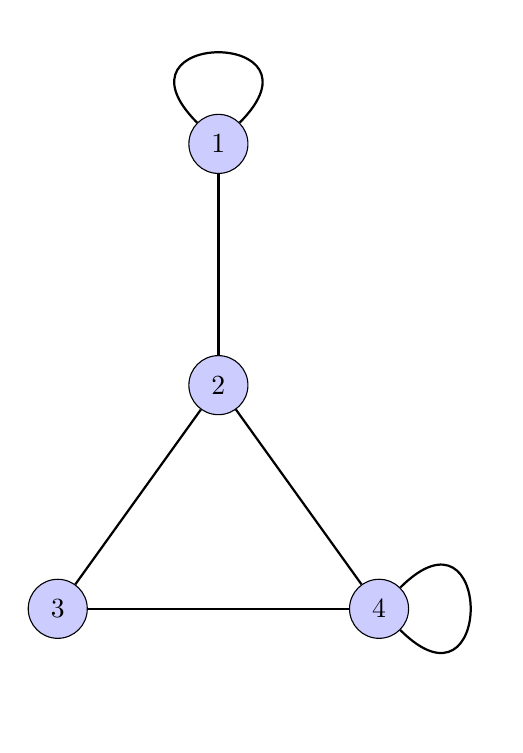
\begin{tikzpicture}[every loop/.style={}]

    \node[main node] (1) {$1$};
    \node[main node] (2) [below = 2.3cm of 1] {$2$};
    \node[main node] (3) [below left = 2.3cm and 1.5cm of 2]  {$3$};
    \node[main node] (4) [below right = 2.3cm and 1.5cm of 2] {$4$};

    \path[draw,thick,-]
    (1) edge node {} (2)
    (2) edge node {} (3)
    (2) edge node {} (4)
    (3) edge node {} (4);

    \path[draw,thick,-]
    (1) edge [loop] (1);

    \path[draw,thick,-]
    (4) edge [in=45, out=-45, loop] (4);

    % \node (4) [circle,draw] {a} edge [in=30,out=60,loop] (4);

\end{tikzpicture}
\end{center}

\vthree

\nin The adjacency matrix for the graph with self-loops is $A =
\mymat{
1 & 1 & 0 & 0 \\
1 & 0 & 1 & 1 \\
0 & 1 & 0 & 1 \\
0 & 1 & 1 & 1 \\
}
$

\clearpage

\nin\Large{\bf Directed Graphs and The Google Matrix}\normalsize
\vspace{4mm}
\hrule

\vthree

\nin Consider a directed graph where the vertices represent pages on the internet.  Directed edges in the graph represent hyperlinks from one page to another.  That is, if there a link from page 1 to page 2 then there is a directed edge in the graph from $v_1$ to $v_2$.

\vthree

\nin Consider the following directed graph

\vthree

\begin{center}
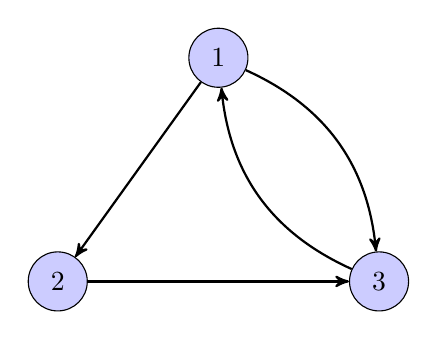
\begin{tikzpicture}

    \node[main node] (1) {$1$};
    \node[main node] (2) [below left = 2.3cm and 1.5cm of 1]  {$2$};
    \node[main node] (3) [below right = 2.3cm and 1.5cm of 1] {$3$};

    \path[draw,thick,->]
    (1) edge node {} (2)
    (2) edge node {} (3)
    (3) edge [bend left] node {} (1)
    (1) edge [bend left] node {} (3);

\end{tikzpicture}
\end{center}

\vthree

\nin The adjacency matrix for a directed graph has a 1 in the $(i,j)$-position if there is a directed edge that starts at $v_i$ and ends at $v_j$:

\[
A_{ij} =
\left\{
\begin{array}{rl}
1 & \textrm{if } i \rightarrow j \\
0 & \textrm{otherwise}
\end{array}
\right.
\]

\vthree

\nin {\bf Example 8}: The adjacency matrix for the graph above is $A =
\mymat{
0 & 1 & 1 \\
0 & 0 & 1 \\
1 & 0 & 0 \\
}
$

\vthree

\nin For directed graphs we can talk about the {\it incoming degree} or {\it outgoing degree} of a vertex.  The incoming degree of a vertex is the number of edges that terminate at the vertex.  Similarly the outgoing degree of a vertex is the number of edges that start at the vertex.  For our purposes, we'll only care about the outgoing degree.

\vthree

\nin The outgoing degrees of the three vertices in the example graph are given by

\[
d_1 = 2 \quad \quad
d_2 = 1 \quad \quad
d_3 = 1
\]

\vthree

\nin Note that the outgoing degree of a vertex is equal to the sum of the associated row in the adjacency matrix.

\vthree

\nin {\bf Def}: The transition matrix of a directed graph $T$ is found by transposing the adjacency matrix and dividing each column by the outgoing degree of the associated vertex.  Mathematically, we have

\[
T_{ij} = \frac{A_{ji}}{d_j}
\]

\vthree

\nin For the example graph, we have

\[
T =
\mymat{
  0 & 0 & 1 \\
1/2 & 0 & 0 \\
1/2 & 1 & 0 \\
}
\]

\vthree

\nin The transition matrix gives us an interesting way of interpreting the graph.  Consider dropping a {\it random walker} on a vertex of the graph.  The walker then moves along a directed edge to another vertex with a probability evenly distributed between each outgoing edges.  For the example graph the probabilities look as follows

\vthree

\begin{center}
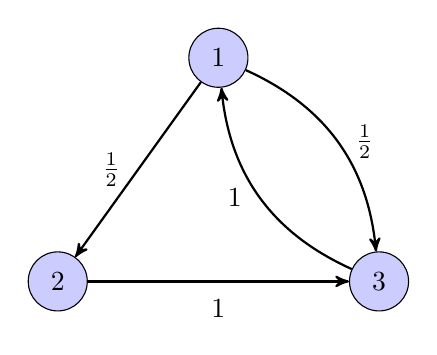
\begin{tikzpicture}

    \node[main node] (1) {$1$};
    \node[main node] (2) [below left = 2.3cm and 1.5cm of 1]  {$2$};
    \node[main node] (3) [below right = 2.3cm and 1.5cm of 1] {$3$};

    \path[draw,thick,->]
    (1) edge node[left,xshift=-1mm]{$\frac{1}{2}$} (2)
    (2) edge node[below,yshift=-1mm]{$1$} (3)
    (3) edge [bend left] node[left,xshift=-1mm]{$1$} (1)
    (1) edge [bend left] node[right,xshift=1mm]{$\frac{1}{2}$} (3);

\end{tikzpicture}
\end{center}

\vthree

\nin Let's see what happens when we drop a random walker at vertex 1 and then let it go.

\vthree

\nin {\bf Step 0}: at $v_1$ with prob $p_1 = 1$

\nin {\bf Step 1}: at $v_2$ with prob $p_2 = 1/2$, at $v_3$ with prob $p_3 = 1/2$

\nin {\bf Step 2}: at $v_1$ with prob $p_1 = 1/2$, at $v_3$ with prob $p_3 = 1/2$

\nin {\bf Step 3}: at $v_1$ with prob $p_1 = 1/2$, at $v_2$ with prob $p_2 = 1/4$, at $v_3$ with prob $p_3 = 1/4$

\vthree

\nin The transition matrix $T$ gives us a way to determine the probabilities of the walker using linear algebra.  Since we begin with the walker at vertex 1 with probability 1 we denote the state of the system by the vector

\[
\bx\iter{0} = \mymat{1 \\ 0 \\ 0}
\]

\vthree

\nin To move the walker one step we multiply the state vector by $T$.  We have

\[
\bx\iter{1} = T\bx\iter{0} =
\mymat{
  0 & 0 & 1 \\
1/2 & 0 & 0 \\
1/2 & 1 & 0 \\
}
\mymat{1 \\ 0 \\ 0}
=
\mymat{0 \\ 1/2 \\ 1/2}
\]

\vthree

\nin Note that the state vector after step one corresponds to the probabilities we deduced above for the random walker.  To get the state of the system after two steps we multiply again by the transition matrix.

\[
\bx\iter{2} = T\bx\iter{1} =
\mymat{
  0 & 0 & 1 \\
1/2 & 0 & 0 \\
1/2 & 1 & 0 \\
}
\mymat{0 \\ 1/2 \\ 1/2}
=
\mymat{1/2 \\ 0 \\ 1/2}
\]

\vthree

\nin which again agrees with the previously computed probabilities.  Taking one more step, we have

\[
\bx\iter{3} = T\bx\iter{2} =
\mymat{
  0 & 0 & 1 \\
1/2 & 0 & 0 \\
1/2 & 1 & 0 \\
}
\mymat{1/2 \\ 0 \\ 1/2}
=
\mymat{1/2 \\ 1/4 \\ 1/4}
\]

\vthree

\nin Now suppose that we let the random walker go for a large number of steps until the state vector no longer changes from step to step.  The resulting vector is as follows

\[
\bx =
\mymat{0.4 \\ 0.2 \\ 0.4}
\]

\vthree

\nin This says that after a large number of time there is a 40\% chance that the walker is at vertex 1, a 20\% chance that it's at vertex 2, and a 40\% chance that it's at vertex 3.

\vthree

\nin It's easy to check that the given vector is an eigenvector of the transition matrix $T$ with associated eigenvalue $\lambda = 1$.

\[
\mymat{
  0 & 0 & 1 \\
0.5 & 0 & 0 \\
0.5 & 1 & 0 \\
}
\mymat{0.4 \\ 0.2 \\ 0.4}
=
\mymat{
0.4 \\
0.2 \\
0.2 + 0.2
}
= \mymat{0.4 \\ 0.2 \\ 0.4}
\]

\vthree

\nin Note that any nonzero scalar multiple of this vector would also be an eigenvector with associated eigenvalue 1.  When we interpret the vector as a probability distribution we always scale the vector so that it has all nonnegative entries that sum to 1.

\vthree

\nin If we return to the analogy that the graph represents a network of webpages, then the eigenvector of interest indicates the long term behavior of a web surfer that is randomly clicking on hyperlinks.  The pages that have high probabilities are deemed more important than the others, and would therefore be displayed higher up in the list by Google.  The eigenvector is called the {\bf PageRank} vector and the $\ith$ entry in the vector is called the PageRank of page $i$.

\vthree

\nin Note that this was a simple case where the transition matrix $T$ was a stochastic matrix (all nonnegative entries with column sums of 1).  But this isn't always the case for every directed graph.

\clearpage

\nin Consider the following digraph

\vthree

\begin{center}
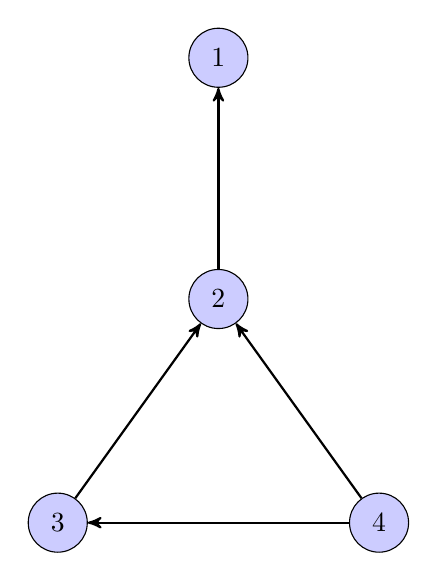
\begin{tikzpicture}

    \node[main node] (1) {$1$};
    \node[main node] (2) [below = 2.3cm of 1] {$2$};
    \node[main node] (3) [below left = 2.3cm and 1.5cm of 2]  {$3$};
    \node[main node] (4) [below right = 2.3cm and 1.5cm of 2] {$4$};

    \path[draw,thick,->]
    (3) edge node {} (2)
    (4) edge node {} (3)
    (4) edge node {} (2)
    (2) edge node {} (1);

\end{tikzpicture}
\end{center}

\vthree

\nin The associated adjacency matrix is $A =
\mymat{
0 & 0 & 0 & 0 \\
1 & 0 & 0 & 0 \\
0 & 1 & 0 & 0 \\
0 & 1 & 1 & 0 \\
}
$

\vthree

\nin The outgoing degrees of the vertices are

\[
d_1 = 0 \quad\quad
d_2 = 1 \quad\quad
d_3 = 1 \quad\quad
d_4 = 2
\]

\vthree

\nin Ignoring the zero outgoing degree of vertex 1, the transition matrix $T$ is given by

\[
T =
\mymat{
0 & 1 & 0 & 0 \\
0 & 0 & 1 & 1/2 \\
0 & 0 & 0 & 1/2 \\
0 & 0 & 0 & 0 \\
}
\]

\vthree

\nin Suppose we start with a random walker at vertex 4.  Then the first several state vectors are

\[
 \bx\iter{0} = \mymat{0 \\ 0 \\ 0 \\ 1}
 \quad
 \bx\iter{1} = T\bx\iter{0} = \mymat{0 \\ 1/2 \\ 1/2 \\ 0}
 \quad
 \bx\iter{2} = T\bx\iter{1} = \mymat{1/2 \\ 1/2 \\ 0 \\ 0}
\]

\vthree

\[
 \bx\iter{3} = T\bx\iter{2} = \mymat{1/2 \\ 0 \\ 0 \\ 0}
 \quad
 \bx\iter{4} = T\bx\iter{3} = \mymat{0 \\ 0 \\ 0 \\ 0}
\]

\clearpage

\nin We immediately see a problem at Step 3.  The resulting state vector is no longer a probability distribution because the entries of the vector don't sum to 1.

\vthree

\nin The problem is that vertex 1 does not have any outgoing nodes, so the probability of the random walker doesn't have anywhere to go and sort of falls off the edge. We call vertex 1 a {\bf dangling vertex} or {\bf dangling node}.

\vthree

\nin Note also that the transition matrix $T$ for the graph with the dangling vertex is not a stochastic matrix.  The column associated with the dangling vertex is all zeros and thus does not sum to 1.

\vthree

\nin OK, so how do we fix this?  Google's solution is to add a directed edge from the dangling vertex to every other vertex in the graph (including itself).  The web analogy is that when a random surfer reaches a dangling node, it jumps randomly to any page in the web with equal probability.  After fixing the dangling node, the directed graph looks as follows

\begin{center}
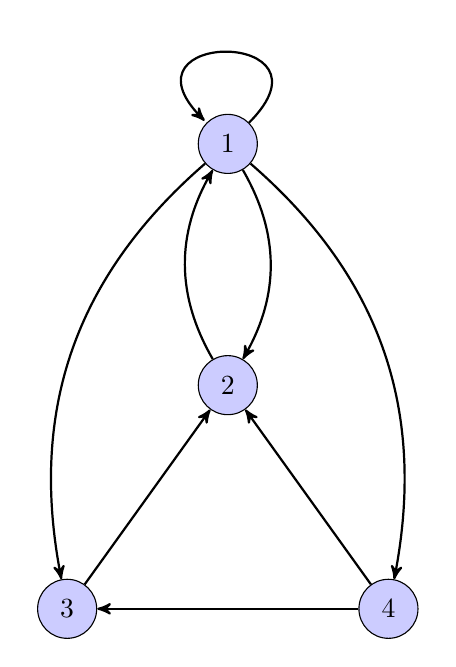
\begin{tikzpicture}

    \node[main node] (1) {$1$};
    \node[main node] (2) [below = 2.3cm of 1] {$2$};
    \node[main node] (3) [below left = 2.3cm and 1.5cm of 2]  {$3$};
    \node[main node] (4) [below right = 2.3cm and 1.5cm of 2] {$4$};

    \path[draw,thick,->]
    (3) edge node {} (2)
    (4) edge node {} (3)
    (4) edge node {} (2)
    (1) edge[bend left] node {} (2)
    (1) edge[bend left] node {} (4)
    (1) edge[bend right] node {} (3)
    (2) edge[bend left] node {} (1);

    \path[draw,thick,-]
    (1) edge [loop] (1);

\end{tikzpicture}
\end{center}

\vthree

\nin The associated transition matrix for the new graph is as follows:

\[
T =
\mymat{
1/4 & 1 & 0 & 0 \\
1/4 & 0 & 1 & 1/2 \\
1/4 & 0 & 0 & 1/2 \\
1/4 & 0 & 0 & 0 \\
}
\]

\vthree

\nin Notice that the new transition matrix is in fact stochastic.  It's PageRank vector is

\[
\bx = \mymat{
0.42 \\
0.32 \\
0.15 \\
0.10
}
\]

\clearpage

\nin OK, so the PageRank vector is the eigenvector associated with eigenvalue $\lambda = 1$.

\vthree

\begin{itemize}
\item How do we know that a stochastic matrix $T$ always has an eigenvalue $\lambda = 1$?
\item How that there isn't an eigenvalue bigger than 1?
\item Are there multiple eigenvectors with associated eigenvalue $\lambda = 1$?
\end{itemize}

\vthree

\nin {\bf Fact 5}: If $T$ is column-stochastic then $\lambda = 1$ is an eigenvalue.

\vthree

\nin Before we can prove this we need to prove an important lemma about eigenvalues.

\vthree

\nin {\bf Lemma}: If $\lambda$ is an eigenvalue of $A$ then it is also an eigenvalue of $A^T$.

\vthree

\nin {\bf Proof}: Recall that the determinant of a matrix and its transpose are the same.  We then have

\[
\det\myp{A - \lambda I} = \det\myp{A - \lambda I}^T = \det\myp{A^T - \lambda I}
\]

\vthree

\nin This means that $A$ and $A^T$ have the same characteristic polynomial.  Since the eigenvalues of a matrix are the roots of its characteristic polynomial it must be the case that the eigenvalues of $A$ and $A^T$ are the same.

\vthree

\nin {\bf Caveat}: Even though the eigenvalues of $A$ and $A^T$ are the same it is usually {\bf NOT} the case that their associated eigenvectors are the same.

\vthree

\nin OK, now we're ready to prove Fact 5.

\vthree

\nin {\bf Proof}: Let ${\bf 1}$ be the vector of all 1's.  Since the columns of $T$ sum to 1 we have

\[
T^T{\bf 1} = {\bf 1} \quad \Rightarrow \quad \lambda = 1 \textrm{ is an eigenvalue of } T \textrm{ and } T^T
\]

\hfill $\square$

\vthree

\nin {\bf Fact 6}: If $T$ is column-stochastic then it has no eigenvalue $\lambda$ such that $\myab{\lambda} > 1$.

\nin {\bf Proof}:  Suppose that $\lambda$ is an eigenvalue of $T$ and $T^T$.  Let $\bw$ be the eigenvector of $T^T$ associated with $\lambda$.  Then we have $T^T\bw = \lambda \bw$.  Suppose that $w_i$ is the largest entry in $\bw$ (in absolute value).  From the equation, we have

\[
\myab{\lambda w_i} = \myab{\sum_j [T^T]_{ij} w_j} = \myab{\sum_j T_{ji} w_j}
\]

\vthree

\nin Note that the sum over $j$ on the right is just the dot product of $\bw$ with the $i^\textrm{th}$ row of $T^T$, which is also the $i^\textrm{th}$ column of $T$.

\nin Next, I'm going to pull the $\lambda$ out of the absolute values on the left.  But the result should still be positive, so I better put an absolute value around the $\lambda$ as well.

\[
\myab{\lambda} \myab{w_i} = \myab{\sum_j T_{ji} w_j}
\]

\vthree

\nin Now, we've assumed that $w_i$ is the largest absolute entry in $\bw$.  Since the term on the right is a dot product of a column of $T$ with $\bw$, and we know that $T$ is column-stochastic, it's easy to see that the largest the right-hand side can be is if the $i^\textrm{th}$ column of $T$ is the vector that has a $1$ in the $i^\textrm{th}$ position, and zeros every else.  If the $i^\textrm{th}$ column of $T$ is any other vector with all nonnegative entries that sums to 1 the expression on the right will be smaller.  Thus we have

\[
\myab{\lambda} \myab{w_i} = \myab{\sum_j T_{ji} w_j} \leq \myab{w_i}
\]

\vthree

\nin Cancelling the $\myab{w_i}$ on both sides of the inequality gives $\myab{\lambda} \leq 1$, which was what we were after.

\hfill $\square$

\vthree

\nin The last question we posed was whether $T$ could have multiple eigenvectors associated with $\lambda = 1$.  This is an important question if we are to interpret the dominant eigenvector as the PageRank vector.  It would be weird if there were multiple PageRank vectors associated with a web.

\vthree

\nin It turns out that there are a couple of cases that can lead to non-unique dominant eigenvectors.  The first is the case when the graph has multiple disconnected components.  We've looked at this case before, so we won't beat it to death again.  The new case is the following:

\vthree

\begin{center}
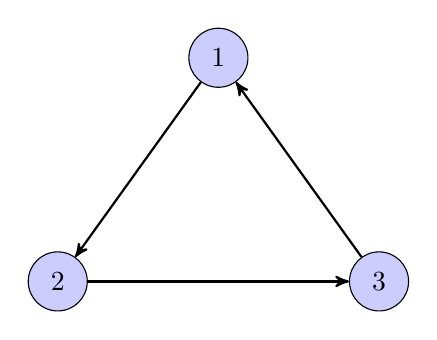
\begin{tikzpicture}

    \node[main node] (1) {$1$};
    \node[main node] (2) [below left = 2.3cm and 1.5cm of 1]  {$2$};
    \node[main node] (3) [below right = 2.3cm and 1.5cm of 1] {$3$};

    \path[draw,thick,->]
    (1) edge node {} (2)
    (2) edge node {} (3)
    (3) edge node {} (1);

\end{tikzpicture}
\end{center}

\vthree

\nin which has transition matrix $T = \mymat{0 & 0 & 1 \\ 1 & 0 & 0 \\ 0 & 1 & 0}$.

\vthree

\nin If we drop a random walker at vertex 1 then we have $\bx\iter{0} = \be_1$.  Then

\[
\bx\iter{1} = T\bx\iter{0} = \be_2 \quad \quad
\bx\iter{2} = T\bx\iter{1} = \be_3 \quad \quad
\bx\iter{3} = T\bx\iter{2} = \be_1
\]

\vthree

\nin It's clear that if we let the walker run for a long time, it will never settle down into a stationary state.  It will instead skip between being located at each of the vertices with probability 1.  When this happens we say that the graph is {\it periodic}.

\vthree

\nin It turns out that the reason this happens is because $T$ has three distinct eigenvalues each with magnitude equal to 1.  They are

\[
\lambda_1 = 1 \quad \quad
\lambda_{2,3} = 0.5 \pm \frac{\sqrt{3}}{2}i \quad \quad
\]

\vthree

\nin OK, so what do we do to avoid these special cases?  Google's solution is to {\bf first fix dangling nodes} to obtain a stochastic matrix $T$  and then add outgoing links from each page to every other page in the web.  This can be justified intuitively by the notion that occasionally web surfers opt to type a new URL into the browser rather than clicking on a hyperlink.  We need to make this modification to the transition matrix in such a way that we still obtained a column-stochastic matrix.  We define the new matrix

\[
G = \myp{1-p}T + p\frac{1}{n}\mathbf{1}\mathbf{1}^T
\]

\vthree

\nin where $\mathbf{1}$ is $n$-dimensional vector of all $1$'s. Notice that $G$ is a column-stochastic matrix as well.  The parameter $p$ is a tuning parameter that sets the probability that the surfer makes a random jump.  The tuning parameter $p$ is usually chosen to be $p = 0.15$.

\vthree

\nin {\bf Computing the PageRank Vector in Practice}

\vthree

\nin OK, so how to we actually compute the PageRank vector (i.e. the eigenvector of $G$ with eigenvalue $\lambda = 1$)?  For very small matrices in class we would row-reduce $G - \lambda I$ to find its nullspace vector.  In practice this is really not a good idea.  Remember that Gaussian-Elimination is an ${\cal O}\myp{n^3}$ method, and if $G$ is a many billions $\times$ many billions matrix, this will pretty much take until the end of time.  Instead we'll compute it using the random walker analogy we talked about in class.  We'll start with a random probability vector as an initial guess, and then apply the matrix $G$ repeatedly to let the random walker move about the graph.  When the entries of the vector (i.e. the probabilities of the locations of the walker) stop changing very much, we'll stop and take that vector as the stationary distribution (i.e. the PageRank vector).

\vthree

\nin This process is actually a very common (although naive) method for finding the eigenvector of a matrix corresponding to it's largest eigenvector.  It's called the {\bf Power Method}, and here's why it works:

\vthree

\nin Let $A$ be a $n \times n$ column-stochastic matrix assume that it has $\lambda_1 = 1$ and all of its other eigenvalues are less than 1.

\[
\lambda_1 = 1 > \myab{\lambda_2} \geq \myab{\lambda_3} \geq \cdots \geq \myab{\lambda_n}
\]

\vthree

\nin Let $\bx\iter{0}$ be a random vector in $\R{n}$.  Since the eigenvectors of $A$ form a basis, we can write

\[
\bx\iter{0} = \alpha_1 \bv_1 + \alpha_2 \bv_2 + \alpha_3 \bv_3 + \cdots + \alpha_n \bv_n
\]

\vthree

\nin for some set of coefficients $\mys{\alpha_i}$. Now define $\bx\iter{1}$ as follows

\beq
\nn \bx\iter{1} = A\bx\iter{0} &=& \alpha_1 A\bv_1 + \alpha_2 A\bv_2 + \alpha_3 A\bv_3 + \cdots + \alpha_n A\bv_n  \\
\nn &=&  \alpha_1 \myp{\lambda_1\bv_1} + \alpha_2 \myp{\lambda_2\bv_2} + \alpha_3 \myp{\lambda_3\bv_3} + \cdots + \alpha_n \myp{\lambda_n\bv_n} \\
\nn &=&  \alpha_1 \bv_1 + \alpha_2 \myp{\lambda_2\bv_2} + \alpha_3 \myp{\lambda_3\bv_3} + \cdots + \alpha_n \myp{\lambda_n\bv_n}
\eeq

\vthree

\nin Similarly

\beq
\nn \bx\iter{2} = A\bx\iter{1} &=&  A\myp{\alpha_1 \bv_1 + \alpha_2 \lambda_2\bv_2 + \alpha_3 \lambda_3\bv_3 + \cdots + \alpha_n \lambda_n\bv_n} \\
\nn  &=&  \alpha_1 A\bv_1 + \alpha_2 \lambda_2A\bv_2 + \alpha_3 \lambda_3A\bv_3 + \cdots + \alpha_n \lambda_nA\bv_n \\
\nn  &=&  \alpha_1 \bv_1 + \alpha_2 \lambda_2^2\bv_2 + \alpha_3 \lambda_3^2\bv_3 + \cdots + \alpha_n \lambda_n^2\bv_n
\eeq

\vthree

\nin  Note that every time we hit the new vector by $A$ again, each eigenvector component gets multiplied again by its eigenvalue.  After $m$ iterations of the method, we have

\beq
\nn \bx\iter{m} = A\bx\iter{m-1} &=&
\alpha_1 \bv_1 + \alpha_2 \lambda_2^m\bv_2 + \alpha_3 \lambda_3^m\bv_3 + \cdots + \alpha_n \lambda_n^m\bv_n
\eeq

\vthree

\nin Remember that we're hoping that the iterate $\bx\iter{m}$ is getting closer and closer to the largest eigenvector, $\bv_1$.  From the above expression it looks like all of the other eigenvectors are hanging around, but you have to think about what happens when you take powers of the eigenvalues.  Since all but the first eigenvalue are smaller than one, powers of the eigenvalues get really small as the iteration goes on.  Eventually, each power of the form $\lambda_j^m$ is so small that their corresponding eigenvectors are not expressed in $\bx\iter{m}$, and $\bx\iter{m}$ is a good approximation of the PageRank vector.

\vthree

\nin Now, you want to be a little careful here.  Even if you started your iteration with a random nonnegative vector that summed to one, roundoff error will probably make it so the iterate is not quite a probability vector anymore.  As such, its usually a good idea to re-scale the vector to make it a probability vector.  You can either do this after each iteration of the Power Method, or at the very end.

\vthree

\nin So why is it called the Power Method?  It turns out that by repeatedly multiplying iterates by $A$, we're implicitly taking powers of the matrix.  Notice that

\[
\bx\iter{m} = A\bx\iter{m-1} = A^2\bx\iter{m-2} = \cdots = A^m\bx\iter{0}
\]

\vthree

\nin So the vector after $m$ iterations is the same (in exact arithmetic) vector you would get if you multiplied the starting vector by the $m^\textrm{th}$ power of $A$.  Of course, we would never do this in practice, because multiplying matrices is together is tremendously more expensive than multiplying matrices by vectors.

\clearpage

\nin OK, so how do we know when we're done?  Remember that we're after the stationary distribution of the random walker.  So one good {\it stopping criterion} is to measure the change between successive iterates and stop when the change is small.  One common way to do this would be to, on the $m^\textrm{th}$ iteration, look at the norm of the difference between $\bx\iter{m}$ and $\bx\iter{m-1}$.  If $\|\bx\iter{m} - \bx\iter{m-1}\|$ is less than some small tolerance (I asked you to use $10^{-5}$ in your homework) then you say the method has converged, and return $\bx\iter{m}$ as the approximation of the PageRank vector.

\vthree

\nin {\bf The Power Method with the Actual Google Matrix}

\vthree

\nin OK, one more trick that we should be aware of when working with the actual Google matrix:

\[
G = \myp{1-p}T + p\frac{1}{n}\mathbf{1}\mathbf{1}^T
\]

\vthree

\nin Notice that the matrix $G$ is really a combination of the original transition matrix $T$ that describes the connections of the web, and the second matrix $\mathbf{1}\mathbf{1}^T/n$ which describes the random teleportations.  The teleportation matrix is a {\it dense} matrix with every entry equal to $1/n$.  On the other hand the matrix $T$ is pretty {\it sparse} because its only nonzero entries correspond to edges between connected vertices.  For the real internet, each webpage is on average connected to only ten other pages.  This means that a typical column of $T$ will have ten nonzero entries, and many billions of zeros.  Clever matrix storage schemes will actually only store the nonzero entries in the matrix, since the zeros won't do anything when the matrix multiplies a vector.  This means that for a, say, billion $\times$ billion matrix, we only have to store ten billion nonzero entries.  If we were to store all of the zeros too, that would require storing $(10^9)^2 = 10^{18}$ entries (I looked it up, that's a {\it quintillion}). Now, if we were to actually add the teleportation matrix to $T$ we'd have to store all $10^{18}$ of those numbers.  This seems like a bad idea.  Let's see how we can multiply $G$ by a probability vector, without actually forming $G$.

\vthree

\nin Let $\bx$ be a vector of nonnegative entries that sum to 1.  Then

\[
G\bx = \myp{1-p}T\bx + \frac{p}{n}\mathbf{1}\mathbf{1}^T\bx
\]

\vthree

\nin Notice in the second term we have $\mathbf{1}^T\bx$.  This is a dot product that acts to sum up the entries of $\bx$, which we know to be 1.  This gives us

\[
G\bx = \myp{1-p}T\bx + \frac{p}{n}\mathbf{1}
\]

\vthree

\nin This expression says that to apply the action of $G$ to a probability vector $\bx$, we can multiply $\bx$ by $\myp{1-p}T$ and then add $p/n$ to each entry in the resultant vector.  This allows us to multply vectors by $G$ without ever forming $G$!  I've asked you to use this trick in your homework when implementing your PageRank function.

\end{document}






















